\begin{figure}[H]
\centering
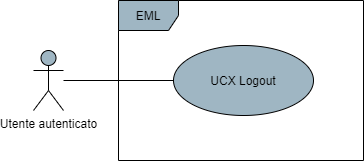
\includegraphics[scale=0.6]{res/UseCase/Immagini/Logout}
\caption{Diagramma UML\ped{G} per modulo di Logout}
\end{figure}

\subsubsection{UC5 - Logout}
\begin{itemize}
\item \textbf{Attori primari}: utente autenticato;
\item \textbf{Descrizione}: l'utente viene sloggato dalla piattaforma;
\item \textbf{Scenario Principale}: l'utente richiede il logout tramite il bottone dedicato;
\item \textbf{Precondizione}: l'utente ha precedentemente effettuato il login ed è attualmente autenticato;
\item \textbf{Postcondizione}: l'utente non è più autenticato.
\end{itemize}